%%%%%%%%%%%%%%%%%%%%%%%%%%%%%%%%%%%%%%%%%
% Focus Beamer Presentation
% LaTeX Template
% Version 1.0 (8/8/18)
%
% This template has been downloaded from:
% http://www.LaTeXTemplates.com
%
% Original author:
% Pasquale Africa (https://github.com/elauksap/focus-beamertheme) with modifications by 
% Vel (vel@LaTeXTemplates.com)
%
% Template license:
% GNU GPL v3.0 License
%
% Important note:
% The bibliography/references need to be compiled with bibtex.
%
%%%%%%%%%%%%%%%%%%%%%%%%%%%%%%%%%%%%%%%%%

%----------------------------------------------------------------------------------------
%	PACKAGES AND OTHER DOCUMENT CONFIGURATIONS
%----------------------------------------------------------------------------------------

\documentclass{beamer}

\usetheme{focus} % Use the Focus theme supplied with the template
% Add option [numbering=none] to disable the footer progress bar
% Add option [numbering=fullbar] to show the footer progress bar as always full with a slide count

% Uncomment to enable the ice-blue theme
%\definecolor{main}{RGB}{92, 138, 168}
%\definecolor{background}{RGB}{240, 247, 255}

%------------------------------------------------

\usepackage{booktabs} % Required for better table rules

%----------------------------------------------------------------------------------------
%	 TITLE SLIDE
%----------------------------------------------------------------------------------------

\usepackage[utf8]{inputenc}
%\usepackage[T2A]{fontenc}
\usepackage[russian]{babel}
%\usepackage{booktabs}


%Библиотеки для Игоря
\usepackage{tikz}
\usetikzlibrary{positioning,arrows}
\usepackage{graphicx} % Allows including images
\usepackage{booktabs}

\title{Суперкомпьютерные технологии \\и основы искусственного интеллекта}

\subtitle{1 - Введение}

\author{Глызин Дмитрий Сергеевич}

\titlegraphic{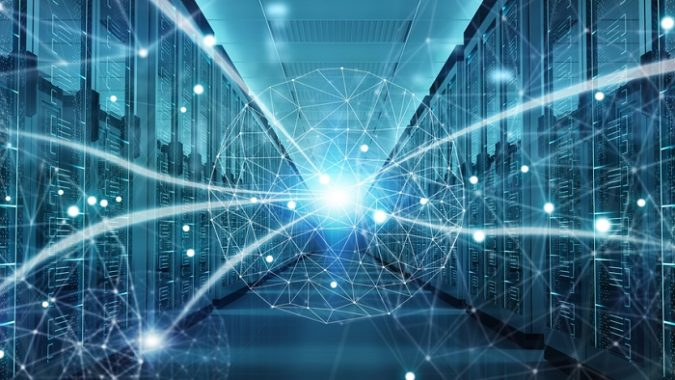
\includegraphics[scale=0.8]{Images/datacenter.jpg}} % Optional title page image, comment this line to remove it

\institute{Ярославский государственный \\университет им. П.Г. Демидова}

\date{13 сентября 2021}

%------------------------------------------------

\begin{document}

%------------------------------------------------

\begin{frame}
	\maketitle % Automatically created using the information in the commands above
\end{frame}

%----------------------------------------------------------------------------------------
%	 SECTION 1
%----------------------------------------------------------------------------------------

\section{HPC, ML, AI} % Section title slide, unnumbered

%------------------------------------------------


\begin{frame}{Top500 - June 2021}
	\begin{table}
		\centering % Centre the table on the slide
\small		
                \begin{tabular}{p{0.1cm} p{8cm} p{0.7cm} p{0.5cm} p{0.5cm}}

			N  &  System & kCr & PF/s & MW\\
			\toprule
			1 &   Supercomputer Fugaku, A64FX 48C 2.2GHz, Tofu interconnect D, Fujitsu 
RIKEN Center for Computational Science Japan &  7,630 & 442 &29\\
			\midrule
			 2 &    Summit - IBM Power System AC922, IBM POWER9 22C 3.07GHz, NVIDIA Volta GV100, Dual-rail Mellanox EDR Infiniband, IBM
DOE/SC/Oak Ridge National Laboratory United States   & 2,414 & 148 &10\\
			\midrule
                            3 &  Sierra - IBM Power System AC922, IBM POWER9 22C 3.1GHz, NVIDIA Volta GV100, Dual-rail Mellanox EDR Infiniband, IBM/NVIDIA/Mellanox DOE/NNSA/LLNL United States  & 1,572 & 94 & 7 \\
			\midrule
			4 &   Sunway TaihuLight - Sunway MPP, Sunway SW26010 260C 1.45GHz, Sunway, NRCPC National Supercomputing Center in Wuxi
			China  &  10,649 & 93 &29\\
		\end{tabular}
	%\caption{Table caption}
	\end{table}
\end{frame}

%------------------------------------------------

\begin{frame}{Top500 - June 2021}
	\begin{table}
		\centering % Centre the table on the slide
\small		
                \begin{tabular}{p{0.1cm} p{8cm} p{0.7cm} p{0.5cm} p{0.5cm}}
			 5 &    Perlmutter - HPE Cray EX235n, AMD EPYC 7763 64C 2.45GHz, NVIDIA A100 SXM4 40 GB, Slingshot-10, HPE DOE/SC/LBNL/NERSC United States    & 706 & 64 &2.5\\
			\midrule
                            6 &  Selene - NVIDIA DGX A100, AMD EPYC 7742 64C 2.25GHz, NVIDIA A100, Mellanox HDR Infiniband, Nvidia NVIDIA Corporation United States & 555 & 63 & 2.6 \\
			\midrule
                            7 &   Tianhe-2A - TH-IVB-FEP Cluster, Intel Xeon E5-2692v2 12C 2.2GHz, TH Express-2, Matrix-2000, NUDT National Super Computer Center in Guangzhou China & 4,981 & 61 & 18 \\
			\midrule
                            8 &   JUWELS Booster Module - Bull Sequana XH2000, AMD EPYC 7402 24C 2.8GHz, NVIDIA A100, Mellanox HDR InfiniBand/ParTec ParaStation ClusterSuite, Atos Forschungszentrum Juelich (FZJ) Germany  & 449 & 44 & 1.7 \\
			
		\end{tabular}
	%\caption{Table caption}
	\end{table}
\end{frame}

%------------------------------------------------

\begin{frame}{Top500 - June 2021}
	\begin{table}
		\centering % Centre the table on the slide
\small		
                \begin{tabular}{p{0.2cm} p{8cm} p{0.7cm} p{0.5cm} p{0.5cm}}
			9 &     	HPC5 - PowerEdge C4140, Xeon Gold 6252 24C 2.1GHz, NVIDIA Tesla V100, Mellanox HDR Infiniband, Dell EMC
Eni S.p.A.  Italy     & 669 & 35 &2.2\\
			\midrule
                            10 &   Frontera - Dell C6420, Xeon Platinum 8280 28C 2.7GHz, Mellanox InfiniBand HDR, Dell EMC Texas Advanced Computing Center/Univ. of Texas United States  & 448 & 23 & ? \\
			\midrule
                            61 &    Christofari - NVIDIA DGX-2, Xeon Platinum 8168 24C 2.7GHz, Mellanox InfiniBand EDR, NVIDIA Tesla V100, Nvidia
SberCloud Russia  & 99 & 6.7 & ?\\
			\midrule
                            199 &     Lomonosov 2 - T-Platform A-Class Cluster, Xeon E5-2697v3 14C 2.6GHz,Intel Xeon Gold 6126, Infiniband FDR, Nvidia K40m/P-100, T-Platforms Moscow State University - Research Computing Center
Russia  & 64 & 2.5 & ? \\
		\end{tabular}
	%\caption{Table caption}
	\end{table}
\end{frame}
%-----------------------------------------------
\begin{frame}[plain]{Igor Slide}
\begin{tikzpicture}[
  minimum size=5mm,
  >=stealth,
  bend angle=45,
  auto]
\node[draw,thick,rectangle,minimum width = 10 cm,text centered ] (Infiniband) at (0,0) {56 Gbit Infiniband};
\node[draw,rectangle,below of=Infiniband,xshift=4.5cm, yshift=-1cm] (dnode14) {\rotatebox[origin=c]{-90}{dnode14}};
\node[draw,rectangle,left of=dnode14] (dnode13) {\rotatebox[origin=c]{-90}{dnode13}};
\node[draw,rectangle,left of=dnode13] (dnode12) {\rotatebox[origin=c]{-90}{dnode12}};
\node[draw,rectangle,left of=dnode12] (dnode11) {\rotatebox[origin=c]{-90}{dnode11}};
\node[draw,rectangle,left of=dnode11] (dnode10) {\rotatebox[origin=c]{-90}{dnode10}};
\node[draw,rectangle,left of=dnode10] (dnode09) {\rotatebox[origin=c]{-90}{dnode09}};
\node[draw,rectangle,left of=dnode09,minimum height = 1.6 cm,minimum width = 1.6 cm,xshift=-0.4cm] (dnode08) {dnode08};
\node[draw,rectangle,left of=dnode08,minimum height = 1.6 cm,minimum width = 1.6 cm,xshift=-1cm] (dnode07) {dnode07};
\node[draw,circle,below of=dnode07,minimum height = 1.8 cm,minimum width = 1.8 cm,yshift=-3cm] (USER) {USER};
\node[draw,rectangle,below of=dnode10,yshift=-3cm,minimum height = 1.6 cm,minimum width = 1.6 cm] (ctrl1) {ctrl1};
\node[draw,rectangle,below of=dnode13,yshift=-3cm,minimum height = 1.6 cm,minimum width = 1.6 cm] (storage1) {storage1};

\node[below of=dnode12,yshift=-1.2cm,minimum height = 1.6 cm,minimum width = 1.6 cm] (bit) {\tiny1Gbit Ethernet};

\draw[->] (Infiniband.south) -| (dnode07.north);
\draw[->] (Infiniband.south) -| (dnode08.north);
\draw[->] (Infiniband.south) -| (dnode09.north);
\draw[->] (Infiniband.south) -| (dnode10.north);
\draw[->] (Infiniband.south) -| (dnode11.north);
\draw[->] (Infiniband.south) -| (dnode12.north);
\draw[->] (Infiniband.south) -| (dnode13.north);
\draw[->] (Infiniband.south) -| (dnode14.north);


\draw[<->, color=red] (dnode08) -- (USER) node[near start, color=black]{\rotatebox[origin=c]{-90}{}};
\draw[<->, color=red] (dnode07) -- +(0,-3) node[near start, color=black]{\rotatebox[origin=c]{-90}{}} -- (USER) ;

\draw[->, color=red] (USER.south)   -- +(0,-0.5) -| (ctrl1) node[near start, color=black]{\tiny ssh -p 2222 
cluster.accelcomp.org} ;

\draw (-5,-4)   -- ++(10,0);
\draw[->] (dnode09) -- +(0,-2);
\draw[->] (dnode10) -- +(0,-2);
\draw[->] (dnode11) -- +(0,-2);
\draw[->] (dnode12) -- +(0,-2);
\draw[->] (dnode13) -- +(0,-2);
\draw[->] (dnode14) -- +(0,-2);
\draw[<->] (storage1) -- +(0,2);
\draw[<->] (ctrl1) -- +(0,2);

\draw[->] (-2.2,-2.8) -- ++(0,-1.2);
\draw[->] (-4.2,-2.8) -- ++(0,-1.2);
\end{tikzpicture}
\end{frame}



%------------------------------------------------

\begin{frame}{Машинное обучение}
	\begin{columns}
		\column{0.5\textwidth}
			Василий Кандинский, "Композиция VIII"
		
		\column{0.5\textwidth}
			\includegraphics[width=\linewidth]{Images/MLfrontpage.png}
	\end{columns}
\end{frame}


%------------------------------------------------

\begin{frame}{Глубокое обучение}
	\begin{columns}
		\column{0.5\textwidth}
			http://introtodeeplearning.com/
		
		\column{0.5\textwidth}
			\includegraphics[width=\linewidth]{Images/MITdl.png}
	\end{columns}
\end{frame}



\end{document}
